% Provenance (never printed): see sources/outline_sources.md (Year 3:
% geophysical fluid dynamics: rotating-frame equations, Rossby number,
% hydrostatic and geostrophic balance, thermal wind, buoyancy frequency).
% Brief: sources/book5/BRIEFS.md, ch. 19. Curves from
% figdata/bachelor-3/inertial_oscillation.py, thermal_wind.py and
% buoyancy_frequency.py. Exercise and problem values in the Book 5 scratch
% calculator calc/ch19.py. The Steppe of Orrin, its lake, its stations and
% its winds are invented.
\chapter{Geofysische vloeistofdynamica}\label{ch:b3:gfd-foundations}

Roer in een kopje thee en de draaiing is binnen een minuut uitgedoofd; de theeblaadjes verzamelen zich in het
midden op de bodem, en verder gebeurt er niets.
Ook de oceaan en de atmosfeer worden geroerd, door de Zon en de wind, maar op een roterende planeet en in
lagen met verschillende dichtheid. Rotatie en gelaagdheid zorgen dat ze zich houden aan
regels die een theekopje nooit laat zien: winden waaien langs de isobaren in plaats van
er dwars op, weigeren kolommen vloeistof te kantelen, en de wind van de bovenste
troposfeer ligt besloten in de temperaturen eronder. Dit hoofdstuk stelt de vergelijkingen op
van deze grote, trage, dunne stromingen en de weinige getallen die
bepalen welke termen ertoe doen.

\begin{recall}
De Coriolis- en centrifugaalkrachten in een roterend assenstelsel, de Navier--Stokes
en continuïteitsvergelijkingen, de viscositeit, het Reynoldsgetal en de hydrostatische
relatie zijn behandeld in de natuurkundeboeken. De Coriolisparameter $f = 2\Omega
\sin\varphi$, de drukgradiëntkracht, het geostrofisch evenwicht, de
geostrofische en \omterm{def:b3:gfd-foundations:gradient}{gradiëntwinden} en de straalstromen worden behandeld in Boek~3,
in het hoofdstuk over de algemene circulatie van de atmosfeer; de
Ekmanlaag in het hoofdstuk over de circulatie van de oceaan; de potentiële
temperatuur, statische stabiliteit en de oscillatie van een opgetild luchtpakketje in
het hoofdstuk over de structuur van de atmosfeer en de oceaan.
\end{recall}

\section{Vergelijkingen in een roterend assenstelsel}\label{sec:b3:gfd-foundations:equations}

In een assenstelsel dat meedraait met de Aarde, met de hoeksnelheid
$\vec\Omega$, voldoet een vloeistofpakketje met snelheid $\vec u$ aan
\[
\frac{\mathrm D\vec u}{\mathrm Dt} + 2\vec\Omega\times\vec u =
-\frac{1}{\rho}\nabla p + \vec g + \nu\nabla^2\vec u ,
\qquad
\frac{\partial\rho}{\partial t} + \nabla\cdot(\rho\vec u) = 0 ,
\]
waarin $\mathrm D/\mathrm Dt = \partial/\partial t + \vec u\cdot\nabla$ de afgeleide
is die het pakketje volgt en $\nu$ de kinematische viscositeit. De
middelpuntvliedende kracht is opgeteld bij de gravitatie: hun som $\vec g$ is de
effectieve zwaarte, loodrecht op de niveauvlakken van de \omterm{def:b3:gravity-geodesy:geopotential}{geopotentiaal}, en
de verticaal wordt daardoor bepaald. Van de rotatie blijft alleen de Coriolisterm, $-2\vec\Omega\times
\vec u$, over, en die verricht geen arbeid: hij draait een pakketje
zonder zijn snelheid te veranderen. De Aarde draait met $\Omega =
\qty{7.292115e-5}{rad/s}$, eenmaal per sterrendag van \qty{23.9345}{h}.
% ledger: geod5:grs80-defining, earth:Trot

Voor bewegingen over afstanden veel kleiner dan de straal $a$ van de Aarde
volstaat een lokaal cartesisch assenstelsel: $x$ naar het oosten, $y$ naar het noorden, $z$ omhoog,
op breedtegraad $\varphi$, het raakvlak van de figuur hieronder. Hier
$\vec\Omega = \Omega\,(0, \cos\varphi, \sin\varphi)$, en de drie
componenten van de impulsvergelijking zijn
\[
\begin{aligned}
\frac{\mathrm Du}{\mathrm Dt} - f v + \tilde f w &= -\frac{1}{\rho}\frac{\partial p}{\partial x} + F_x ,\\
\frac{\mathrm Dv}{\mathrm Dt} + f u &= -\frac{1}{\rho}\frac{\partial p}{\partial y} + F_y ,\\
\frac{\mathrm Dw}{\mathrm Dt} - \tilde f u &= -\frac{1}{\rho}\frac{\partial p}{\partial z} - g + F_z ,
\end{aligned}
\qquad f = 2\Omega\sin\varphi,\quad \tilde f = 2\Omega\cos\varphi ,
\]
met $\vec F$ de wrijving. Voor de dunne, bijna horizontale stromingen van de
oceaan en de atmosfeer vallen de termen in $\tilde f$ weg: $\tilde f w$
is klein naast $fv$ omdat $w \ll v$, en $\tilde f u$ is een tienduizendste
van $g$ (uit \cref{exo:b3:gfd-foundations:5}). De Coriolis-kracht werkt dan alleen
horizontaal, via de lokale verticale component van de rotatie,
$\Omega\sin\varphi$.

\begin{definition}[$f$-vlak en $\beta$-vlak]\label{def:b3:gfd-foundations:planes}
Nabij een referentiebreedtegraad $\varphi_0$ neemt de \emph{$f$-vlak}\index{f-vlak@$f$-vlak}-benadering
de Coriolisparameter als constant aan, $f = f_0 =
2\Omega\sin\varphi_0$. De \emph{$\beta$-vlak}\index{beta-vlak@$\beta$-vlak}-benadering
houdt de eerste-orde verandering met de noordwaartse afstand $y$ in rekening:
$f = f_0 + \beta y$, met $\beta = \mathrm df/\mathrm dy = 2\Omega
\cos\varphi_0/a$.
\end{definition}

Bij \ang{45}, met de gemiddelde straal $a = \qty{6371}{km}$, $f_0 =
\qty{1.031e-4}{s^{-1}}$ en $\beta = \qty{1.62e-11}{m^{-1}.s^{-1}}$: over
\qty{1000}{km} breedtegraad verandert $f$ met \qty{16}{\percent}. Het $f$-vlak
is geschikt voor bewegingen die veel kleiner zijn dan dat; het $\beta$-vlak is nodig voor
stromingen op bekkenschaal en planetaire golven.
% ledger: earth:Rmean, geod5:grs80-defining (values in figdata/bachelor-3/inertial_oscillation.py)

\begin{omfigure}
\begin{minipage}[c]{0.42\linewidth}\centering
\begin{tikzpicture}[>=stealth, font=\small]
\draw[thick] (0,0) circle (2);
\draw[black!40, dashed] (-2,0) -- (2,0);
\draw[->, thick] (0,-2.4) -- (0,2.75) node[above] {$\vec\Omega$};
\draw (0,0) -- (30:2) coordinate (P);
\draw (0.6,0) arc (0:30:0.6);
\node at (15:0.9) {$\varphi$};
\draw[black!60] ($(P)+(120:-1.1)$) -- ($(P)+(120:1.3)$);
\draw[->, omThm, thick] (P) -- ++(0,1.6) node[right] {$\vec\Omega$};
\draw[->, omDef, thick] (P) -- ++(30:0.8) node[anchor=south west, align=left, inner sep=1pt] {$\Omega\sin\varphi$,\\ omhoog};
\draw[->, omMeth, thick] (P) -- ++(120:1.386) node[anchor=south, align=center, inner sep=1pt] {$\Omega\cos\varphi$,\\ noord};
\draw[black!50, densely dotted] ($(P)+(30:0.8)$) -- ($(P)+(0,1.6)$) -- ($(P)+(120:1.386)$);
\draw (P) circle (0.09); \draw ($(P)+(-0.064,-0.064)$) -- ($(P)+(0.064,0.064)$);
\draw ($(P)+(-0.064,0.064)$) -- ($(P)+(0.064,-0.064)$);
\node[font=\scriptsize, anchor=west] at ($(P)+(0.14,-0.03)$) {$x$, oost};
\node[font=\scriptsize, black!60] at (-1.15,-0.25) {evenaar};
\end{tikzpicture}
\end{minipage}\hfill
\begin{minipage}[c]{0.55\linewidth}\centering
\begin{tikzpicture}
\begin{axis}[width=\linewidth, height=0.72\linewidth, xmin=0, xmax=90, ymin=0, ymax=1.8,
  xlabel={breedtegraad (\unit{\degree})}, ylabel={$f$ ($10^{-4}$\,\unit{s^{-1}})},
  xtick={0,15,30,45,60,75,90}, tick label style={font=\scriptsize}, label style={font=\small},
  legend style={font=\scriptsize, draw=none, fill=none}, legend pos=north west]
% computed in figdata/bachelor-3/inertial_oscillation.py
\addplot[omDef, thick] table[x=lat, y=f] {figdata/out/bachelor-3-inertial_oscillation-fbeta.dat};
\addplot[omThm, densely dashed] table[x=lat, y=fb] {figdata/out/bachelor-3-inertial_oscillation-fbeta.dat};
\addplot[only marks, mark=*, mark size=1.6pt] coordinates {(45,1.03126)};
\legend{$2\Omega\sin\varphi$, $\beta$-vlak bij \ang{45}}
\end{axis}
\end{tikzpicture}
\end{minipage}

\par\smallskip{\small Links: het lokale assenstelsel op breedtegraad $\varphi$: $z$
langs de lokale verticaal, $y$ naar het noorden in het raakvlak, $x$ naar het oosten
het papier in. De rotatievector splitst in $\Omega\sin\varphi$ om de
verticaal, die horizontale beweging draait, en $\Omega\cos\varphi$ om de
noordelijke as, die bij dunne stromingen wordt weggelaten. Rechts: de Coriolisparameter en
zijn raaklijn in het $\beta$-vlak bij \ang{45}: dicht bij die breedte over een band van breedtegraden, ver
ervan af bij de evenaar en de pool.}\label{fig:b3:gfd-foundations:frame}
\end{omfigure}
% ledger: geod5:grs80-defining, earth:Rmean

Twee verdere benaderingen vereenvoudigen de vergelijkingen zonder wat ertoe doet te verliezen.
De eerste betreft de dichtheid.

\begin{definition}[Boussinesq-benadering]\label{def:b3:gfd-foundations:boussinesq}
De \emph{Boussinesq-benadering}\index{Boussinesq-benadering} schrijft
de dichtheid als $\rho = \rho_0 + \rho'$, met $\rho_0$ een constante en
$|\rho'| \ll \rho_0$, en houdt $\rho'$ alleen waar die met $g$ is vermenigvuldigd.
De continuïteitsvergelijking wordt $\nabla\cdot\vec u = 0$, en de
impulsvergelijking
\[
\frac{\mathrm D\vec u}{\mathrm Dt} + f\,\vec k\times\vec u =
-\frac{1}{\rho_0}\nabla p' + b\,\vec k + \nu\nabla^2\vec u ,
\qquad b = -g\,\frac{\rho'}{\rho_0} ,
\]
waarbij $p'$ de afwijking van de druk is van de hydrostatische druk
van de dichtheid $\rho_0$, $\vec k$ de naar boven gerichte eenheidsvector en $b$ het
drijfvermogen.
\end{definition}

In de oceaan is $\rho'$ enkele \unit{kg/m^3} op \num{1025}, een fractie van een
procent, en de benadering is uitstekend. In de atmosfeer neemt de dichtheid
met een factor $e$ af over ongeveer \qty{8.5}{km}; de benadering geldt voor
lagen die veel dunner zijn dan dat, en diepere stromingen vervangen $\rho_0$ door een
gemiddeld profiel $\rho_0(z)$, met dezelfde fysica.
% ledger: earth:Hscale

De tweede betreft de verticale richting. Een vloeistof in rust bevindt zich in hydrostatisch
evenwicht; een bewegende vloeistof behoudt dat, met zeer goede benadering, wanneer de
beweging veel breder is dan ze diep is.

\begin{definition}[Hydrostatische benadering]\label{def:b3:gfd-foundations:hydrostatic}
De \emph{hydrostatische benadering}\index{hydrostatische benadering}
vervangt de verticale impulsvergelijking van een bewegende vloeistof door de
hydrostatische relatie, $\partial p/\partial z = -\rho g$.
\end{definition}

\begin{proposition}[Wanneer de hydrostatische benadering geldt]\label{prop:b3:gfd-foundations:hydrostatic}
Voor een beweging met horizontale schaal $L$, diepte $H$ en snelheid $U$, met een
\omterm{def:b3:gfd-foundations:numbers}{Rossby-getal} $U/(fL)$ van hooguit de orde één, is de verticale versnelling
kleiner dan de verticale gradiënt van de drukstoring met een factor
van de orde $(U/fL)\,(H/L)^2$.
\end{proposition}

\begin{proof}
Wanneer de Corioliskracht minstens zo groot is als de versnelling, de
horizontale impulsvergelijking balanceert de horizontale drukgradiënt
daartegen: $p'/(\rho_0 L) \sim fU$, dus $p'/\rho_0 \sim fUL$, en de verticale
gradiënt is $p'/(\rho_0 H) \sim fUL/H$. Continuïteit, $\partial w/\partial z
= -(\partial u/\partial x + \partial v/\partial y)$, begrenst de verticale
snelheid door $W \sim UH/L$, en de verticale versnelling door
$\mathrm Dw/\mathrm Dt \sim UW/L = U^2H/L^2$. De verhouding is $(U^2H/L^2)/(fUL/H)
= (U/fL)(H/L)^2$.
\end{proof}

Een weersysteem van \qty{1000}{km} breed in een troposfeer van \qty{10}{km} diep heeft
$(H/L)^2 = 10^{-4}$ en een \omterm{def:b3:gfd-foundations:numbers}{Rossby-getal} van ongeveer 0.1: de fout van de
\omterm{def:b3:gfd-foundations:hydrostatic}{hydrostatische benadering} is van de orde $10^{-5}$. Ze faalt alleen bij smalle, diepe bewegingen: een
opwaartse stroming in een onweersbui, een convectieve pluim in de oceaan.

\section{Schalen van roterende stroming}\label{sec:b3:gfd-foundations:scales}

Welke termen van de impulsvergelijking ertoe doen, wordt bepaald door twee verhoudingen.

\begin{definition}[Rossby- en Ekmangetal]\label{def:b3:gfd-foundations:numbers}
Voor een stroming met snelheid $U$, horizontale schaal $L$ en diepte $H$ op een planeet met
Coriolisparameter $f$ is het \emph{Rossby-getal}\index{Rossby-getal}
$\mathrm{Ro} = U/(fL)$, de verhouding van de versnelling, van de orde $U^2/L$,
tot de Corioliskracht, van de orde $fU$. Het
\emph{Ekmangetal}\index{Ekmangetal} is $\mathrm{Ek} = \nu/(fH^2)$, de verhouding van de
viskeuze kracht, van de orde $\nu U/H^2$, tot de Corioliskracht; in een
turbulente stroming wordt $\nu$ vervangen door een wervelviscositeit.
\end{definition}

Een badkuip die leegloopt met \qty{0.1}{m/s} over \qty{0.3}{m} heeft een \omterm{def:b3:gfd-foundations:numbers}{Rossby-getal} van
enkele duizenden: de rotatie van de Aarde bepaalt niet de draairichting van de
wervel. Een depressie van \qty{1000}{km} breed met winden van \qty{15}{m/s} heeft
$\mathrm{Ro} \approx 0.14$, en een oceaangyre $\mathrm{Ro} \sim 10^{-4}$.
Viscositeit is nog zwakker: de moleculaire viscositeit van water is
\qty{e-6}{m^2/s}, en de wervelviscositeiten die voor de turbulentie
van de oceaan, \qtyrange{e-5}{e-3}{m^2/s} in de verticale richting, geven
$\mathrm{Ek} \sim 10^{-5}$ over \qty{1000}{m} diepte. De twee getallen hangen
samen met het Reynoldsgetal via $\mathrm{Re} = UL/\nu =
(\mathrm{Ro}/\mathrm{Ek})(L/H)^2$.
% ledger: stewart:eddy (problem values in calc/ch19.py)

Wanneer beide getallen klein zijn, houdt de stationaire horizontale impulsvergelijking
alleen de Corioliskracht en de drukgradiënt over: de stroming is in
geostrofisch evenwicht, $f\,\vec k\times\vec u_g = -(1/\rho)\nabla_h p$, zoals
Boek~3 uit het eerste jaar aan de hand van weerkaarten afleidt. Geostrofie is de limiet
$\mathrm{Ro}, \mathrm{Ek}\to 0$; de correcties daarop zijn van de orde
$\mathrm{Ro}$, en wrijving werkt alleen in dunne lagen met een relatieve dikte van
$\sqrt{\mathrm{Ek}}$, de Ekmanlagen onderaan de atmosfeer en
bovenaan en onderaan de oceaan. Op een $f$-vlak heeft de geostrofische snelheid
geen horizontale divergentie: $\partial u_g/\partial x + \partial
v_g/\partial y = -(1/\rho f)(\partial^2 p/\partial x\partial y -
\partial^2 p/\partial y\partial x) = 0$ voor uniforme $\rho$.

De tegenovergestelde limiet, rotatie zonder drukgradiënt, is de eenvoudigste
beweging die een roterende vloeistof kan maken.

\begin{definition}[Traagheidsoscillatie]\label{def:b3:gfd-foundations:inertial}
Een \emph{traagheidsoscillatie}\index{traagheidsoscillatie} is de
horizontale beweging van een vloeistof waarop geen horizontale kracht werkt behalve de
Coriolisskracht.
\end{definition}

\begin{theorem}[Traagheidscirkels]\label{thm:b3:gfd-foundations:inertial}
Op een $f$-vlak behoudt een pakketje dat met snelheid $U$ in beweging is gebracht,
waarop geen horizontale kracht werkt behalve de Coriolisskracht, zijn snelheid
en beschrijft het een cirkel met straal $U/|f|$, met de klok mee op het noordelijk halfrond en
tegen de klok in op het zuidelijk halfrond, in de traagheidsperiode $2\pi/|f|$, wat de helft
van een siderische dag gedeeld door $\sin\varphi$ is.
\end{theorem}

\begin{proof}
De vergelijkingen zijn $\mathrm du/\mathrm dt = fv$, $\mathrm dv/\mathrm dt =
-fu$. Met $w = u + \mathrm iv$ luiden ze $\mathrm dw/\mathrm dt = -\mathrm
if\,w$, dus $w = U\,\mathrm e^{-\mathrm ift}$ voor een begin naar het oosten: de
snelheid $|w| = U$ blijft constant en de snelheidsvector draait met hoeksnelheid $f$,
met de klok mee wanneer $f > 0$. Door integratie loopt de positie $x + \mathrm iy =
(\mathrm iU/f)(\mathrm e^{-\mathrm ift} - 1)$ rond het punt
$-\mathrm iU/f$ op afstand $U/|f|$. De periode is $2\pi/|f| =
2\pi/(2\Omega|\sin\varphi|)$, en $2\pi/\Omega$ is de siderische dag.
\end{proof}

Op \ang{45} bedraagt de traagheidsperiode \qty{16.9}{h}, en een stroming van
\qty{0.2}{m/s} draait op een cirkel van \qty{1.94}{km}; op \ang{30} is de periode
precies een siderische dag, en op de evenaar zijn er geen traagheidscirkels.
Nadat een storm de oppervlaktelaag van de oceaan in beweging heeft gebracht en vervolgens is weggeëbd,
doet het water precies dat. Drijvende boeien met drijfanker op \qty{15}{m} in de
Noord-Pacifische Oceaan traceerden dagenlang lussen na een storm in oktober 1987, meegevoerd
door de gemiddelde stroming: het derde pad van de onderstaande figuur, na de
cirkel en de spiraal.
% ledger: stewart:inertial, earth:Trot (values in figdata/bachelor-3/inertial_oscillation.py)

\begin{omfigure}
\begin{tikzpicture}
\begin{axis}[width=\linewidth, axis equal image, xmin=-3, xmax=18.5, ymin=-4.6, ymax=1.2,
  xlabel={oostelijke afstand (km)}, ylabel={noordelijke afstand (km)},
  tick label style={font=\scriptsize}, label style={font=\small},
  legend style={font=\scriptsize, draw=none, fill=white, fill opacity=0.85, text opacity=1},
  legend pos=south east, legend columns=3]
% computed in figdata/bachelor-3/inertial_oscillation.py
\addplot[black!45, line width=1.6pt] table[x=x, y=y] {figdata/out/bachelor-3-inertial_oscillation-circle.dat};
\addplot[omDef, thick] table[x=x, y=y] {figdata/out/bachelor-3-inertial_oscillation-spiral.dat};
\addplot[omThm, thick] table[x=x, y=y] {figdata/out/bachelor-3-inertial_oscillation-loops.dat};
\addplot[only marks, mark=*, mark size=1.8pt] coordinates {(0,0)};
\legend{zonder wrijving, wrijving, wrijving en stroming}
\end{axis}
\end{tikzpicture}

\par\smallskip{\small Paden over vier dagen van een pakketje dat met
\qty{0.2}{m/s} naar het oosten beweegt op \ang{45} NB (stip), zonder kracht behalve de
Coriolisskracht: een cirkel met straal \qty{1.94}{km}, met de klok mee doorlopen elke
\qty{16.9}{h} (grijs); met een wrijving die de snelheid halveert in
\num{2.8}~dagen, een naar binnen gerichte spiraal (blauw); hetzelfde pakketje meegevoerd door
een constante naar het oosten gerichte stroming van \qty{0.05}{m/s}, een reeks krimpende lussen
(rood).}\label{fig:b3:gfd-foundations:inertial}
\end{omfigure}
% ledger: stewart:inertial

Tussen geostrofie en de traagheidscirkel ligt de stroming rond een centrum van
hoge of lage druk, waar de isobaren gekromd zijn en de versnelling naar het
centrum niet langer verwaarloosbaar is.

\begin{definition}[Gradiëntwind]\label{def:b3:gfd-foundations:gradient}
De \emph{gradiëntwind}\index{gradiëntwind} is de stationaire, wrijvingsvrije
stroming langs gekromde isobaren, waarin de drukgradiëntkracht, de
Coriolisskracht en de centripetale versnelling elkaar in evenwicht houden.
\end{definition}

\begin{proposition}[De krommingscorrectie]\label{prop:b3:gfd-foundations:gradient}
Laat de isobaren cirkels met straal $r$ zijn op het noordelijk halfrond, en
$V_g$ de geostrofische snelheid die hun drukgradiënt zou geven, met
$\mathrm{Ro}_g = V_g/(fr)$. Rond een lagedrukgebied is de \omterm{def:b3:gfd-foundations:gradient}{gradiëntwind}
$V = 2V_g/(1 + \sqrt{1 + 4\mathrm{Ro}_g})$, trager dan $V_g$; rond een hogedrukgebied
is $V = 2V_g/(1 + \sqrt{1 - 4\mathrm{Ro}_g})$, sneller, en die bestaat alleen
als $\mathrm{Ro}_g \le 1/4$. In eerste orde geldt $V = V_g(1 \mp \mathrm{Ro}_g)$.
\end{proposition}

\begin{proof}
Rond een lagedrukgebied draait de wind tegen de klok in; de drukgradiëntkracht
$fV_g$ wijst naar het centrum, de Coriolisskracht $fV$ naar buiten, en hun
verschil levert de centripetale versnelling: $fV_g - fV = V^2/r$. De positieve
wortel van $V^2 + frV - frV_g = 0$ is $V = (fr/2)(\sqrt{1 +
4\mathrm{Ro}_g} - 1)$; vermenigvuldigen met $(\sqrt{1 + 4\mathrm{Ro}_g} +
1)/(\sqrt{1 + 4\mathrm{Ro}_g} + 1)$ geeft de formule. Rond een hogedrukgebied
draait de wind met de klok mee en wijst de Coriolisskracht naar binnen: $fV - fV_g =
V^2/r$, dus $V^2 - frV + frV_g = 0$, wat alleen reële wortels heeft als $f^2r^2
\ge 4frV_g$; de wortel die naar $V_g$ gaat wanneer $\mathrm{Ro}_g \to 0$ is
$V = (fr/2)(1 - \sqrt{1 - 4\mathrm{Ro}_g})$. Door de wortels te ontwikkelen
geldt $V = V_g(1 \mp \mathrm{Ro}_g + \dots)$.
\end{proof}

Het \omterm{def:b3:gfd-foundations:numbers}{Rossby-getal} van de isobaren meet de correctie: een tiende voor een
depressie van matige omvang. De voorwaarde $\mathrm{Ro}_g \le 1/4$ verklaart waarom het
centrum van een anticycloon zwakke gradiënten en lichte winden heeft, terwijl dat
van een depressie steile gradiënten en stormen kan bevatten.

\section{Rotatie zonder stratificatie}\label{sec:b3:gfd-foundations:taylor}

Een roterende vloeistof van uniforme dichtheid gedraagt zich bij langzame beweging
alsof ze uit starre kolommen bestaat die evenwijdig aan de rotatieas lopen.

\begin{theorem}[Taylor--Proudman]\label{thm:b3:gfd-foundations:taylor-proudman}
In een stationaire stroming van een niet-viskeuze vloeistof van uniforme dichtheid, die roteert
met $\vec\Omega$, met klein \omterm{def:b3:gfd-foundations:numbers}{Rossby-getal}, varieert de snelheid niet langs de richting van de
rotatieas: $(\vec\Omega\cdot\nabla)\vec u = 0$.
\end{theorem}
\index{Taylor--Proudman-stelling}

\begin{proof}
Voor $\mathrm{Ro}\to 0$, stationair en niet-viskeus reduceert de impulsvergelijking
tot $2\vec\Omega\times\vec u = -\nabla(p/\rho_0 + \Phi)$, met $\Phi$ het
\omterm{def:b3:gravity-geodesy:geopotential}{geopotentiaal}. De rotatie van een gradiënt is nul, dus $\nabla\times(\vec\Omega
\times\vec u) = 0$. Voor een constante $\vec\Omega$ is deze rotatie gelijk aan $\vec\Omega
(\nabla\cdot\vec u) - (\vec\Omega\cdot\nabla)\vec u$, en $\nabla\cdot\vec u
= 0$ bij uniforme dichtheid.
\end{proof}

Met $\vec\Omega$ langs $z$ geldt $\partial\vec u/\partial z = 0$: alle drie de
snelheidscomponenten zijn op elke hoogte gelijk. Als een starre bodem daar $w$
verbiedt, geldt $w = 0$ overal, en de horizontale stroming is op elk niveau
gelijk. Een obstakel op de bodem van een roterende tank voelt men daarom tot
aan het oppervlak: de vloeistof erboven kan er niet overheen klimmen, want dat
zou een kolom uitrekken of samendrukken, en ze stroomt op elke hoogte eromheen.
De vloeistofkolom die boven het obstakel blijft staan, is een \emph{Taylorkolom}
\index{Taylorkolom}.

\begin{omfigure}
\begin{tikzpicture}[>=stealth, font=\small]
% side view
\fill[omDef!8] (0,0) rectangle (5.4,3);
\fill[black!10] (2.1,0) rectangle (3.3,3);
\draw[thick] (0,3.3) -- (0,0) -- (5.4,0) -- (5.4,3.3);
\draw[black!50] (0,3) -- (5.4,3);
\draw[fill=black!45] (2.1,0) .. controls (2.4,0.55) and (3.0,0.55) .. (3.3,0) -- cycle;
\draw[black!60, densely dashed] (2.1,0) -- (2.1,3) (3.3,0) -- (3.3,3);
\foreach \y in {0.8,1.6,2.4} {\draw[->, omDef, thick] (0.3,\y) -- (1.9,\y);
  \draw[->, omDef, thick] (3.5,\y) -- (5.1,\y);}
\draw[->, thick, omThm] (2.7,3.25) -- (2.7,4.0) node[right] {$\vec\Omega$};
\node[font=\scriptsize, align=center] at (2.7,1.7) {Taylorkolom};
\node[font=\scriptsize, anchor=north] at (2.7,-0.05) {obstakel};
\node[font=\small] at (2.7,-0.6) {(a) zijaanzicht};
% top view
\begin{scope}[xshift=6.4cm]
\fill[omDef!8] (0,0) rectangle (5.4,3);
\draw[thick] (0,0) rectangle (5.4,3);
\fill[black!10] (2.7,1.5) circle (0.5);
\draw[black!60, densely dashed] (2.7,1.5) circle (0.5);
\foreach \d/\h in {0.3/0.10, 0.75/0.35, 1.2/0.58} {
  \draw[->, omDef, thick] (0.2,1.5+\d) .. controls (1.6,1.5+\d) and (2.0,1.5+\h+0.62) .. (2.7,1.5+\h+0.62)
     .. controls (3.4,1.5+\h+0.62) and (3.8,1.5+\d) .. (5.2,1.5+\d);
  \draw[->, omDef, thick] (0.2,1.5-\d) .. controls (1.6,1.5-\d) and (2.0,1.5-\h-0.62) .. (2.7,1.5-\h-0.62)
     .. controls (3.4,1.5-\h-0.62) and (3.8,1.5-\d) .. (5.2,1.5-\d);}
\node[font=\small] at (2.7,-0.6) {(b) gezien van bovenaf, op elke hoogte};
\end{scope}
\end{tikzpicture}

\par\smallskip{\small Een \omterm{thm:b3:gfd-foundations:taylor-proudman}{Taylorkolom} (schematisch). (a) In een tank met
uniform water dat snel roteert, stuit een langzame stroming op een lage hindernis op de
bodem; de vloeistof boven het obstakel (grijs) blijft op zijn plaats tot aan het
oppervlak, en de stroming op elke hoogte gaat om de kolom heen alsof het obstakel de
bovenkant bereikt. (b) De stroming gezien van bovenaf is op elk
niveau gelijk.}\label{fig:b3:gfd-foundations:taylor}
\end{omfigure}

De atmosfeer en de oceaan zijn gelaagd, en stratificatie verzacht de beperking:
een gestratificeerde vloeistof kan met de hoogte variëren, zoals de stelling
van de \omterm{thm:b3:gfd-foundations:thermal-wind}{thermische wind} voorschrijft.

\section{Stratificatie en de thermische wind}\label{sec:b3:gfd-foundations:stratification}

Het deel van Boek~3 uit het eerste jaar liet een luchtpakketje in een stabiele
atmosfeer opstijgen en vond dat het rond zijn niveau oscilleert. Hetzelfde geldt
in elke gestratificeerde vloeistof, en de frequentie van de oscillatie is de maat

\begin{definition}[Drijfvermogenfrequentie]\label{def:b3:gfd-foundations:buoyancy}
De \emph{drijfvermogenfrequentie}\index{drijfvermogenfrequentie} $N$ van een vloeistof in
rust wordt gedefinieerd door
\[
N^2 = \frac{g}{\theta}\frac{\mathrm d\theta}{\mathrm dz}\ \text{(lucht)},
\qquad
N^2 = -\frac{g}{\rho_0}\frac{\mathrm d\rho_\theta}{\mathrm dz}\ \text{(zeewater)},
\]
waarin $\theta$ de potentiële temperatuur van de lucht is en $\rho_\theta$ de
potentiële dichtheid van het water, de dichtheid die het zou krijgen als het
adiabatisch naar een referentiedruk wordt gebracht.
\end{definition}

\begin{theorem}[Oscillatie van een verplaatst pakketje]\label{thm:b3:gfd-foundations:buoyancy}
Een pakketje dat verticaal over een kleine afstand $\zeta$ uit zijn niveau in een
vloeistof in rust is verplaatst, adiabatisch en zonder menging, gehoorzaamt aan $\ddot\zeta =
-N^2\zeta$. Als $N^2 > 0$ oscilleert het met de hoekfrequentie $N$; als
$N^2 < 0$ groeit de verplaatsing en is de vloeistof instabiel.
\end{theorem}

\begin{proof}
Adiabatisch en zonder menging verplaatst, behoudt het pakketje zijn potentiële
dichtheid $\rho_\theta(z_0)$. Op het niveau $z_0 + \zeta$ heeft het de druk van
zijn omgeving, waarvan de potentiële dichtheid $\rho_\theta(z_0) +
\zeta\,\mathrm d\rho_\theta/\mathrm dz$ is; twee pakketjes bij dezelfde druk
verschillen in dichtheid met het verschil van hun potentiële dichtheden, tot op
de eerste orde. De drijfkracht per massa-eenheid is $-g(\rho_p - \rho_e)/\rho_0 =
g\,\zeta\,(\mathrm d\rho_\theta/\mathrm dz)/\rho_0 = -N^2\zeta$. Voor lucht bij
een gegeven druk varieert de dichtheid als $1/\theta$, dus $-\mathrm
d\rho_\theta/\rho_0 = \mathrm d\theta/\theta$ en komen de twee vormen van $N^2$
overeen.
\end{proof}

In de troposfeer van de standaardatmosfeer, die afkoelt met
\qty{6.49}{K/km} tegenover de \qty{9.77}{K/km} van de droge adiabaat ($g/c_p$,
met $c_p = \gamma R/(\gamma - 1)$, $\gamma = 1.4$ en $R =
\qty{286.9}{J.kg^{-1}.K^{-1}}$), bedraagt $N$ gemiddeld \qty{0.0113}{s^{-1}}, een periode
van \qty{9.3}{min}; in de isotherme onderste stratosfeer is het
\qty{0.0210}{s^{-1}}. In de oceaan heeft de waterkolom van de Noord-Atlantische Oceaan
op \ang{40.5}~NB, \ang{30.5}~WL in het jaargemiddelde de sterkste
stratificatie in de seizoenspycnocline, $N = \qty{0.0106}{s^{-1}}$ op
ongeveer \qty{30}{m}, zes cycli per uur, en veel zwakkere waarden daaronder: hooguit
een paar cycli per uur, zoals waargenomen over de bovenste oceaan.
% ledger: nasa:grc-atmos, nasa:grc-gamma-b5, nws:dalr, data:b5-woa23-atlantic, unesco44:eos80-b5, stewart:stability (values in figdata/bachelor-3/buoyancy_frequency.py)

\begin{omfigure}
\begin{tikzpicture}
\begin{groupplot}[group style={group size=2 by 1, horizontal sep=1.7cm},
  width=0.48\linewidth, height=0.50\linewidth, tick label style={font=\scriptsize},
  label style={font=\small}]
\nextgroupplot[xlabel={$N$ ($10^{-2}$\,\unit{s^{-1}})}, ylabel={hoogte (km)},
  xmin=0, xmax=3, ymin=0, ymax=30, title={\small atmosfeer}]
% computed in figdata/bachelor-3/buoyancy_frequency.py
\addplot[omDef, thick] table[x expr=\thisrow{N}*100, y=z] {figdata/out/bachelor-3-buoyancy_frequency-atm.dat};
\addplot[black!50, densely dashed, domain=0:3, samples=2] {11};
\node[font=\scriptsize, anchor=south east] at (axis cs:2.95,11) {tropopauze};
\nextgroupplot[xlabel={$N$ (cycli per uur)}, ylabel={diepte (m)}, y dir=reverse,
  xmin=0, xmax=7, ymin=0, ymax=2000, title={\small oceaan, \ang{40.5} NB \ang{30.5} WL},
  scaled y ticks=false, ytick={0,500,1000,1500,2000}, yticklabels={0,500,1000,1500,2000}]
\addplot[omThm, thick, mark=*, mark size=0.9pt] table[x=cph, y=z] {figdata/out/bachelor-3-buoyancy_frequency-ocean.dat};
\end{groupplot}
\end{tikzpicture}

\par\smallskip{\small \omterm{def:b3:gfd-foundations:buoyancy}{Drijfvermogenfrequentie}. Links, de standaardatmosfeer:
vrijwel uniform in de troposfeer, in de isotherme onderste
stratosfeer twee keer zo groot, en nog groter boven \qty{25}{km}, waar de temperatuur stijgt.
Rechts, een jaargemiddelde kolom van de Noord-Atlantische Oceaan (temperatuur en
zoutgehalte uit de World Ocean Atlas 2023, potentiële dichtheid uit EOS-80):
een scherp maximum in de seizoenspycnocline, zwakke stratificatie
daaronder.}\label{fig:b3:gfd-foundations:buoyancy}
\end{omfigure}
% ledger: nasa:grc-atmos, data:b5-woa23-atlantic, unesco44:eos80-b5

Stratificatie laat de stroming met de hoogte variëren, en hoe ze dat doet hangt
ervan af of de oppervlakken van constante dichtheid samenvallen met die van
constante druk.

\begin{definition}[Barotrope en barokliene vloeistoffen]\label{def:b3:gfd-foundations:baroclinic}
Een vloeistof is \emph{barotroop}\index{barotrope vloeistof} als haar dichtheid
alleen een functie van de druk is, zodat oppervlakken van constante dichtheid samenvallen
met oppervlakken van constante druk; ze is
\emph{baroklien}\index{barokliene vloeistof} als ze elkaar kruisen.
\end{definition}

In de atmosfeer maakt een horizontale temperatuurgradiënt langs een drukvlak
de lucht \omterm{def:b3:gfd-foundations:baroclinic}{baroklien}. Hydrostatisch evenwicht zorgt er dan voor dat de
drukvlakken met de hoogte steiler gaan hellen, en geostrofisch evenwicht
zet de groeiende helling om in een groeiende wind.

\begin{omfigure}
\begin{tikzpicture}[>=stealth, font=\small, x=1.15cm, y=0.85cm]
\shade[left color=omThm!22, right color=omDef!22] (0,0) rectangle (8,4);
\draw[thick] (0,0) -- (8,0);
\foreach \k/\lab in {1/p_1, 2/p_2, 3/p_3, 4/p_4} {
  \draw[black, thick] (0,0.9*\k) -- (8,0.675*\k) node[right] {$\lab$};}
\foreach \k/\r in {1/0.07, 2/0.11, 3/0.15, 4/0.19} {
  \draw[omMeth, thick, fill=white] (4,0.7875*\k) circle (\r);
  \fill[omMeth] (4,0.7875*\k) circle (0.035);}
\node[font=\scriptsize, anchor=south west] at (4.12,3.3) {$u_g$};
 \node[font=\scriptsize] at (0.8,3.8) {warm};
\node[font=\scriptsize] at (7.2,3.8) {koud};
\draw[->] (0.3,-0.35) -- (2.0,-0.35) node[right, font=\scriptsize] {noord, $y$};
\end{tikzpicture}

\par\smallskip{\small De meetkunde van de \omterm{thm:b3:gfd-foundations:thermal-wind}{thermische wind} (schematisch, een
meridionale doorsnede met de warme kant naar het zuiden, $p_1 > p_2 > p_3 >
p_4$). Warme lucht zet uit, zodat de laag tussen twee drukvlakken
aan de warme kant dikker is dan aan de koude kant: elk vlak helt
steiler naar de koude kant dan het vlak eronder. De geostrofische
wind is evenredig met de helling en neemt toe met de hoogte (cirkels, groter
bij sterkere wind), naar het oosten, uit het
vlak.}\label{fig:b3:gfd-foundations:geometry}
\end{omfigure}

\begin{theorem}[Thermische wind]\label{thm:b3:gfd-foundations:thermal-wind}
In een atmosfeer in hydrostatisch en geostrofisch evenwicht varieert de geostrofische
wind met de druk als
\[
\frac{\partial u_g}{\partial\ln p} = \frac{R}{f}\left(\frac{\partial T}{\partial y}\right)_p ,
\qquad
\frac{\partial v_g}{\partial\ln p} = -\frac{R}{f}\left(\frac{\partial T}{\partial x}\right)_p .
\]
Tussen twee drukniveaus $p_b > p_t$ is de \emph{thermische
wind}\index{thermische wind}, het verschil van de geostrofische winden, luidt
\[
\vec u_g(p_t) - \vec u_g(p_b) = \frac{R}{f}\,\ln\frac{p_b}{p_t}\;\vec k\times\nabla_p\bar T ,
\]
waarin $\bar T$ de gemiddelde temperatuur van de laag is: hij waait langs de
isothermen van de laag, met de koude lucht links in het
noordelijk halfrond.
\end{theorem}

\begin{proof}
Op een oppervlak van constante druk geldt $\mathrm dp = (\partial p/\partial y)
\,\mathrm dy + (\partial p/\partial z)\,\mathrm dz = 0$, en met
$\partial p/\partial z = -\rho g$ voldoet de hoogte $z_p$ van het oppervlak aan
$g\,\partial z_p/\partial y = (1/\rho)\,\partial p/\partial y$. In termen van
de \omterm{def:b3:gravity-geodesy:geopotential}{geopotentiaal} $\Phi = gz_p$ van het oppervlak luidt het geostrofisch evenwicht
$fu_g = -\partial\Phi/\partial y$ en $fv_g = \partial\Phi/\partial x$, met
de afgeleiden genomen langs het oppervlak. De hydrostatische relatie en de
ideale gaswet geven $\partial\Phi/\partial p = -1/\rho = -RT/p$, dat wil zeggen
$\partial\Phi/\partial\ln p = -RT$. Door $fu_g =
-\partial\Phi/\partial y$ naar $\ln p$ te differentiëren volgt $f\,\partial
u_g/\partial\ln p = R\,\partial T/\partial y$, en analoog voor $v_g$.
Bij integratie van $p_b$ naar $p_t$ neemt $\ln p$ af met $\ln(p_b/p_t)$, dus
$u_g(p_t) - u_g(p_b) = -(R/f)\ln(p_b/p_t)\,\partial\bar T/\partial y$, en
$v_g(p_t) - v_g(p_b) = (R/f)\ln(p_b/p_t)\,\partial\bar T/\partial x$: dit zijn de
componenten van de vectorvorm, aangezien $\vec k\times\nabla\bar T =
(-\partial\bar T/\partial y, \partial\bar T/\partial x)$.
\end{proof}

\begin{corollary}[Thermische wind in hoogte]\label{cor:b3:gfd-foundations:thermal-wind-z}
In hoogtecoördinaten, voor de atmosfeer, $\partial u_g/\partial z =
-(g/fT)\,\partial T/\partial y + (u_g/T)\,\partial T/\partial z$; voor de
oceaan in de \omterm{def:b3:gfd-foundations:boussinesq}{Boussinesq-benadering} geldt $\partial u_g/\partial z =
(g/f\rho_0)\,\partial\rho/\partial y$ en $\partial v_g/\partial z =
-(g/f\rho_0)\,\partial\rho/\partial x$.
\end{corollary}

\begin{proof}
In de lucht, $fu_g = -(1/\rho)\partial p/\partial y = -RT\,\partial\ln
p/\partial y$ en $\partial\ln p/\partial z = -g/(RT)$. Dan
\[
f\,\frac{\partial(u_g/T)}{\partial z} = -R\,\frac{\partial}{\partial y}\frac{\partial\ln p}{\partial z}
= g\,\frac{\partial(1/T)}{\partial y} = -\frac{g}{T^2}\frac{\partial T}{\partial y} ,
\]
Uitwerking van het linkerlid geeft de formule. In de oceaan, $fu_g = -(1/\rho_0)\partial
p/\partial y$ en $\partial p/\partial z = -\rho g$, dus $f\,\partial u_g/
\partial z = (g/\rho_0)\,\partial\rho/\partial y$; evenzo voor $v_g$.
\end{proof}

De tweede term van de atmosferische vorm, die voortkomt uit de afname van de temperatuur
met de hoogte, is kleiner dan de eerste en verdwijnt in een isotherme
laag; geïntegreerd over een laag met haar gemiddelde temperatuur, geeft de eerste term
alleen bijna de drukvorm, aangezien $\Delta z \approx (R\bar T/g)
\ln(p_b/p_t)$ (Probleem, deel~IV). In de oceaan zet dezelfde stelling een
doorsnede van de dichtheid over een stroom om in de verticale afschuiving: de basis van
de dynamische methode van de oceanografen.


De straalstromen uit Boek~3 zijn \omterm{thm:b3:gfd-foundations:thermal-wind}{thermische winden}. In het zonaal gemiddelde
van januari 1991--2020 neemt de westenwind op \ang{30}~NB toe van
\qty{4.3}{m/s} op \qty{850}{hPa} tot \qty{40.4}{m/s} op \qty{250}{hPa}; met
$f$ op \ang{30} en $R$ is deze afschuiving het kenmerk van een laag waarvan de gemiddelde
temperatuur daalt naar het noorden met \qty{7.5}{K} per \qty{1000}{km}. Op \ang{45}
NB levert de afschuiving van \qtyrange{6.0}{23.2}{m/s} een daling van \qty{5.0}{K} per
\qty{1000}{km}. De figuur hieronder toont de profielen en, voor elke breedtegraad,
de temperatuurdaling naar de pool, afgelezen uit de afschuiving: het grootst in de
subtropen van het winterhalfrond, waar de subtropische straalstroom
zich bevindt, \qty{43.9}{m/s} op \qty{200}{hPa} en \ang{30}~NB in januari en
\qty{41.0}{m/s} op \ang{30}~ZB in juli. Boven \qty{200}{hPa} op \ang{30}~NB
neemt de wind weer af: de stelling van de \omterm{thm:b3:gfd-foundations:thermal-wind}{thermische wind}, achterstevoren gelezen, zegt dat
daar, in de onderste stratosfeer, stijgt de temperatuur naar de pool toe.
% ledger: data:b5-ncep-uwnd, nasa:grc-atmos (values in figdata/bachelor-3/thermal_wind.py)

\begin{omfigure}
\begin{tikzpicture}
\begin{groupplot}[group style={group size=2 by 1, horizontal sep=1.7cm},
  width=0.48\linewidth, height=0.46\linewidth, tick label style={font=\scriptsize},
  label style={font=\small}, legend style={font=\scriptsize, draw=none, fill=none}]
\nextgroupplot[xlabel={$\bar u$ (\unit{m/s})}, ylabel={druk (\unit{hPa})}, ymode=log,
  y dir=reverse, xmin=0, xmax=50, ymin=100, ymax=1000, ytick={1000,850,700,500,300,200,100},
  yticklabels={1000,850,700,500,300,200,100}, legend pos=south east, title={\small januari}]
% computed in figdata/bachelor-3/thermal_wind.py
\addplot[omThm, thick, mark=*, mark size=1pt] table[x=u, y=p] {figdata/out/bachelor-3-thermal_wind-prof-30.dat};
\addplot[omDef, thick, mark=square*, mark size=1pt] table[x=u, y=p] {figdata/out/bachelor-3-thermal_wind-prof-45.dat};
\addplot[omMeth, thick, mark=triangle*, mark size=1.3pt] table[x=u, y=p] {figdata/out/bachelor-3-thermal_wind-prof-60.dat};
\legend{\ang{30}~NB, \ang{45}~NB, \ang{60}~NB}
\nextgroupplot[xlabel={breedtegraad (\unit{\degree})}, ylabel={daling naar de pool (K/\qty{1000}{km})},
  xmin=-80, xmax=80, ymin=0, ymax=8, xtick={-80,-40,0,40,80}, legend cell align=left,
  legend style={at={(axis cs:0,0.15)}, anchor=south},
  title={\small \qtyrange{850}{250}{hPa}}]
\addplot[omDef, thick, restrict x to domain=-90:-20] table[x=lat, y=drop] {figdata/out/bachelor-3-thermal_wind-grad-jan.dat};
\addplot[omThm, thick, restrict x to domain=-90:-20] table[x=lat, y=drop] {figdata/out/bachelor-3-thermal_wind-grad-jul.dat};
\addplot[omDef, thick, restrict x to domain=20:90, forget plot] table[x=lat, y=drop] {figdata/out/bachelor-3-thermal_wind-grad-jan.dat};
\addplot[omThm, thick, restrict x to domain=20:90, forget plot] table[x=lat, y=drop] {figdata/out/bachelor-3-thermal_wind-grad-jul.dat};
\legend{januari, juli}
\end{groupplot}
\end{tikzpicture}

\par\smallskip{\small Links, de zonaal gemiddelde zonale wind in januari
(NCEP--NCAR Reanalysis~1, gemiddelde 1991--2020) op drie breedtegraden: de wind
neemt toe met de hoogte door de troposfeer. Rechts, de laaggemiddelde
temperatuurdaling naar de pool tussen \qty{850}{hPa} en
\qty{250}{hPa}, afgelezen uit de windafschuiving met de stelling van de \omterm{thm:b3:gfd-foundations:thermal-wind}{thermische wind}
(equatorwaarts van \ang{25}, waar de geostrofie faalt, weggelaten): groter op het
winterhalfrond.}\label{fig:b3:gfd-foundations:jets}
\end{omfigure}
% ledger: data:b5-ncep-uwnd

\section{De Rossby-deformatiestraal}\label{sec:b3:gfd-foundations:rossby-radius}

Rotatie en stratificatie leggen elk een schaal op; samen leggen ze
een lengte vast.

\begin{definition}[Rossby-deformatiestraal]\label{def:b3:gfd-foundations:rossby-radius}
De \emph{Rossby-deformatiestraal}\index{Rossby-deformatiestraal}
van een laag van diepte $H$ en \omterm{def:b3:gfd-foundations:buoyancy}{drijfvermogenfrequentie} $N$ is $L_R = NH/|f|$.
\end{definition}

\begin{proposition}[Potentiële en kinetische energie van gebalanceerde stroming]\label{prop:b3:gfd-foundations:rossby-radius}
In een hydrostatische, geostrofische stroming met horizontale schaal $L$ in een laag van
diepte $H$ en \omterm{def:b3:gfd-foundations:buoyancy}{drijfvermogenfrequentie} $N$ is de verhouding van de potentiële energie
opgeslagen in de verplaatste dichtheidsoppervlakken tot de kinetische energie
van de orde $(L/L_R)^2$.
\end{proposition}

\begin{proof}
Geostrofie geeft de drukstoring $p'/\rho_0 \sim fUL$; de
hydrostatische betrekking geeft het drijfvermogen $b \sim p'/(\rho_0H) \sim fUL/H$. Een
drijfvermogen $b$ in een vloeistof met \omterm{def:b3:gfd-foundations:buoyancy}{drijfvermogenfrequentie} $N$ betekent dat dichtheidsoppervlakken
verticaal verplaatst over $\eta = b/N^2$; zulke oppervlakken slaan per
massa-eenheid van de orde $N^2\eta^2 = b^2/N^2 \sim f^2U^2L^2/(N^2H^2)$. Gedeeld
door de kinetische energie, van de orde $U^2$, is dit $(fL/NH)^2 = (L/L_R)^2$.
\end{proof}

Bewegingen veel breder dan $L_R$ bevatten het grootste deel van hun energie in gekantelde
dichtheidsoppervlakken, bewegingen veel smaller in hun snelheid; bij $L_R$ zijn de twee
gelijk, en de instabiliteit van barokliene stromingen, die zich voedt met de
potentiële energie van de gekantelde oppervlakken, groeit het snelst rond die schaal. Voor
de troposfeer, met het gemiddelde $N$ van de standaardatmosfeer, $H =
\qty{11}{km}$ en $f$ op \ang{45}, $L_R = \qty{1210}{km}$: de schaal van de
depressies en anticyclonen op een weerkaart. Voor de bovenste kilometer van
de Noord-Atlantische waterkolom op \ang{40.5}~NB, $L_R = \qty{38}{km}$, dertig
keer kleiner: de oceaan heeft zijn eigen weer, wervels van tientallen kilometers
breed, en een model dat ze oplost heeft een veel fijner rooster nodig. Op schalen
nabij $L_R$ verandert $f$ met $\beta L_R/f$, \qty{19}{\percent} voor de
atmosfeer en minder dan één procent voor de oceaan: oceaanwervels leven op een
$f$-vlak, weersystemen voelen het $\beta$-vlak.
% ledger: nasa:grc-atmos, data:b5-woa23-atlantic, earth:Rmean (values in figdata/bachelor-3/buoyancy_frequency.py)

\begin{inthelab}[Een planeet op een draaitafel]
\begin{minipage}[t]{0.52\linewidth}\vspace{0pt}
In een laboratorium voor geofysische vloeistofdynamica staat een bak water op een
draaitafel; een camera draait mee en ziet het water zoals een waarnemer op een
planeet het zou zien. Vóór elke proef laat men het water spin-up ondergaan totdat het
als een star lichaam meedraait; dat duurt enkele minuten, vele omwentelingen van de tafel. Daarna
brengen de onderzoekers kleurstof in, of verschuiven ze langzaam een obstakel over de bodem:
de kleurstof stijgt in een verticale kolom boven het obstakel en de stroming splitst zich
op elk niveau rond het obstakel. Met een laag zoet water boven zout water, of met een
verwarmde buitenwand en een gekoeld centrum, wordt de bak \omterm{def:b3:gfd-foundations:baroclinic}{baroklien}, en
verschijnen straalstromen, wervels en meanderende fronten, waarvan de grootte
de \omterm{def:b3:gfd-foundations:rossby-radius}{Rossby-deformatiestraal} van de bak voorspelt.
\end{minipage}\hfill
\begin{minipage}[t]{0.44\linewidth}\vspace{0pt}
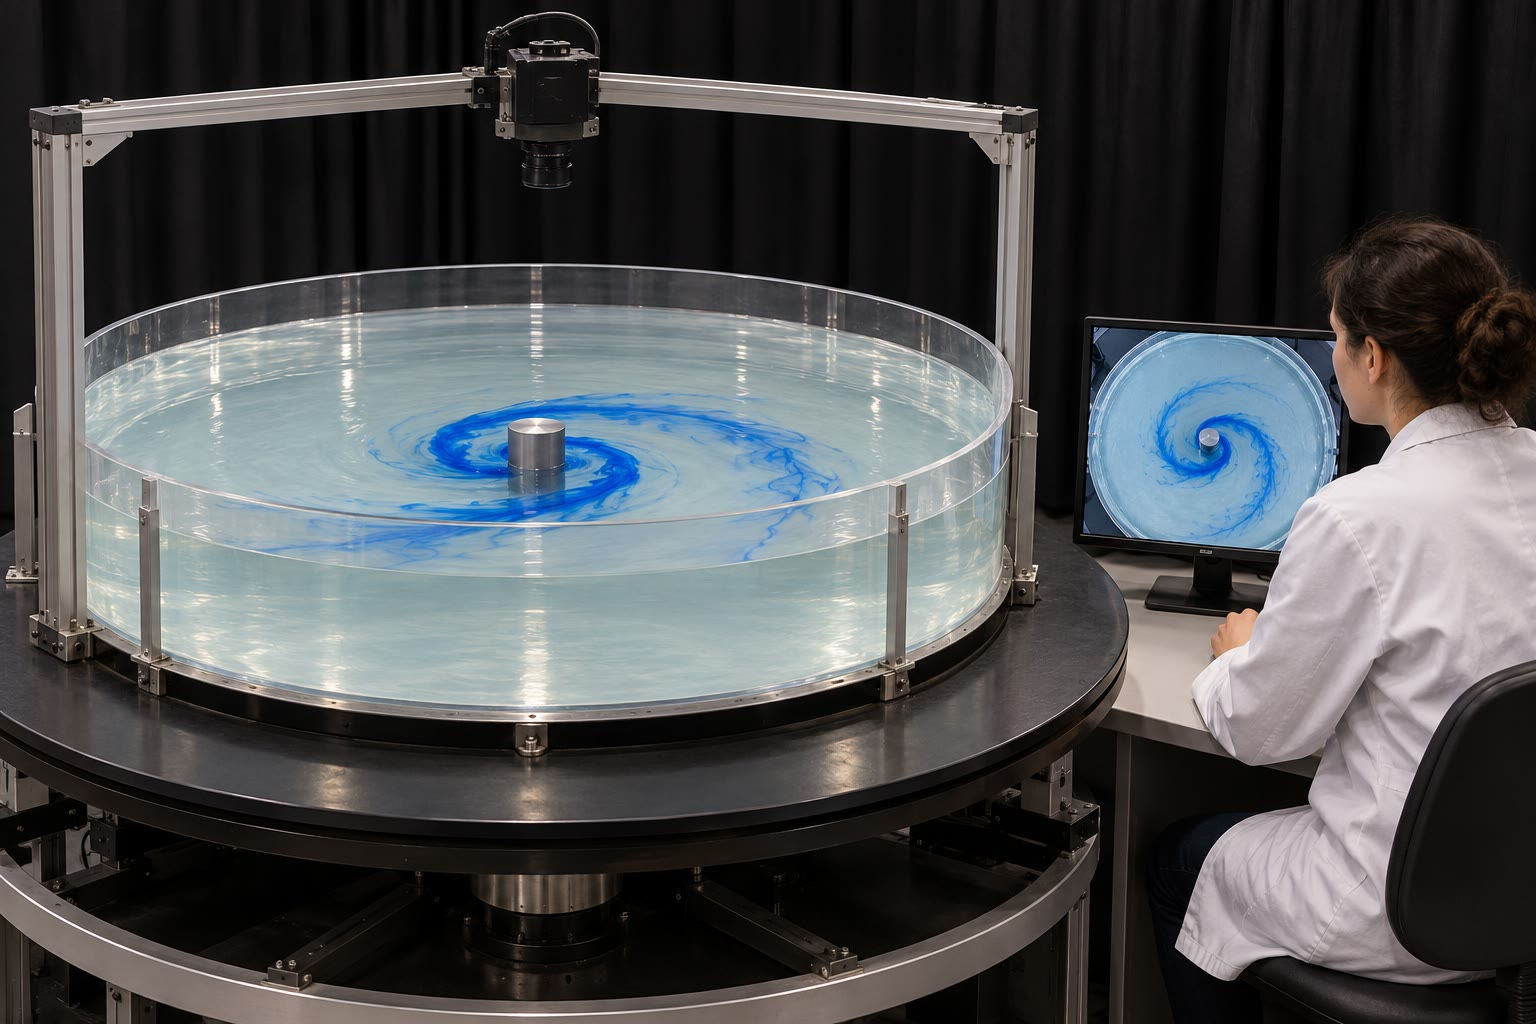
\includegraphics[width=\linewidth]{images/book5/ai/b3-rotating-tank.jpg}

{\scriptsize Een roterende bak: kleurstof die spiraalvormig rond een cilinder draait, gefilmd door een
camera die met de tafel meedraait (Door AI gegenereerde illustratie).}
\end{minipage}
\end{inthelab}

\section{Oefeningen}

\begin{exercise}[$\star$]\label{exo:b3:gfd-foundations:1}
Neem $\Omega = \qty{7.292115e-5}{rad/s}$. (a)~Bereken de
Coriolisparameter en de traagheidsperiode op \ang{30}, \ang{45} en \ang{60} NB.
(b)~Bereken de straal van de traagheidscirkel van een stroom van
\qty{0.20}{m/s} op dezelfde breedtegraden. (c)~Vergelijk de traagheidsperiode op
\ang{30} met de sterrendag, \qty{23.9345}{h}.
\end{exercise}

\begin{exercise}[$\star$]\label{exo:b3:gfd-foundations:2}
Bereken op \ang{45} NB het \omterm{def:b3:gfd-foundations:numbers}{Rossby-getal} van een stofduivel (\qty{10}{m/s},
\qty{10}{m}), een zeebries (\qty{5}{m/s}, \qty{20}{km}),
een depressie (\qty{15}{m/s}, \qty{1000}{km}) en een oceaangyre (\qty{0.05}{m/s},
\qty{2000}{km}). Welke daarvan liggen dicht bij het geostrofisch evenwicht?
\end{exercise}

\begin{exercise}[$\star$]\label{exo:b3:gfd-foundations:3}
Op \ang{45} NB neemt de gemiddelde temperatuur van de troposfeer, \qty{250}{K},
naar het noorden af met \qty{5}{K} per \qty{1000}{km}. Bereken met de eerste term van de
\omterm{thm:b3:gfd-foundations:thermal-wind}{thermische wind} in de hoogte de verticale verschuiving van de westenwind en
de toename van de wind over \qty{10}{km}.
\end{exercise}

\begin{exercise}[$\star$]\label{exo:b3:gfd-foundations:4}
De stabiliteit $E = -(1/\rho)\,\mathrm d\rho_\theta/\mathrm dz$ van de bovenste
kilometer van de oceaan ligt tussen \num{50e-8} en \qty{1000e-8}{m^{-1}};
in diepe geulen is ze \qty{e-8}{m^{-1}}. Bereken $N = \sqrt{gE}$, de
periode van de drijfvermogenoscillatie en $N$ in cycli per uur voor deze
drie waarden.
\end{exercise}

\begin{exercise}[$\star\star$]\label{exo:b3:gfd-foundations:5}
Een weersysteem heeft $U = \qty{10}{m/s}$, $L = \qty{1000}{km}$, $H =
\qty{10}{km}$, op \ang{45} NB. (a)~Schat de verticale snelheid en de
verticale versnelling ervan, en vergelijk die laatste met $g$ en met de
verticale gradiënt van de drukstoring, $fUL/H$. (b)~Bereken de
weggelaten Coriolisterm $\tilde fu$ en vergelijk die met $g$.
\end{exercise}

\begin{exercise}[$\star\star$]\label{exo:b3:gfd-foundations:6}
Neem $f = \qty{e-4}{s^{-1}}$ en cirkelvormige isobaren met een straal van
\qty{300}{km}. (a)~De drukgradiënt rond een lagedrukgebied geeft $V_g =
\qty{20}{m/s}$: bereken de \omterm{def:b3:gfd-foundations:gradient}{gradiëntwind}. (b)~Rond een hogedrukgebied,
$V_g = \qty{5}{m/s}$: bereken de \omterm{def:b3:gfd-foundations:gradient}{gradiëntwind}. (c)~Wat is de grootste
$V_g$ die rond het hogedrukgebied mogelijk is, en wat is dan de wind?
\end{exercise}

\begin{exercise}[$\star\star$]\label{exo:b3:gfd-foundations:7}
Een bak van \qty{20}{cm} diep draait eenmaal per \qty{6}{s}; het water erin heeft $\nu =
\qty{e-6}{m^2/s}$. (a)~Bereken $f = 2\Omega$, vervolgens het \omterm{def:b3:gfd-foundations:numbers}{Rossby-getal} van een
stroming van \qty{1}{cm/s} langs een cilinder van \qty{5}{cm} breed, en het \omterm{def:b3:gfd-foundations:numbers}{Ekmangetal}
van de bak. Zal er een \omterm{thm:b3:gfd-foundations:taylor-proudman}{Taylorkolom} ontstaan? (b)~De theorie geeft een
spin-uptijd $H/\sqrt{\nu\Omega}$: bereken die in minuten en in omwentelingen van de tafel.
\end{exercise}

\begin{exercise}[$\star\star$]\label{exo:b3:gfd-foundations:8}
In het januari-zonaal gemiddelde van 1991--2020 is de westenwind \qty{4.27}{m/s}
op \qty{850}{hPa} en \qty{40.39}{m/s} op \qty{250}{hPa} op \ang{30} NB,
\qty{5.99}{m/s} en \qty{23.17}{m/s} op \ang{45} NB. Met $R =
\qty{286.9}{J.kg^{-1}.K^{-1}}$, bereken de meridionale gradiënt van de
gemiddelde temperatuur van de laag op beide breedtegraden, en verklaar waarom de
straalstroom op \ang{30} NB sterker is.
\end{exercise}

\begin{exercise}[$\star\star$]\label{exo:b3:gfd-foundations:9}
(a)~Bereken de \omterm{def:b3:gfd-foundations:rossby-radius}{Rossby-deformatiestraal} van de troposfeer ($N =
\qty{0.0113}{s^{-1}}$, $H = \qty{11}{km}$, \ang{45} NB) en van de bovenste
oceaan ($N = \qty{0.00357}{s^{-1}}$, $H = \qty{1000}{m}$, \ang{40.5} NB).
(b)~Met $a = \qty{6371}{km}$ bereken $\beta$ op beide breedtegraden en de
relatieve verandering $\beta L_R/f$ van de Coriolisparameter over elke straal.
\end{exercise}

\begin{exercise}[$\star\star\star$]\label{exo:b3:gfd-foundations:10}
Een waterpakketje van het oppervlaktewater dat met $U$ beweegt, wordt afgeremd door een lineaire
wrijving: $\mathrm du/\mathrm dt = fv - ru$, $\mathrm dv/\mathrm dt = -fu -
rv$. (a)~Los op met $w = u + \mathrm iv$ en beschrijf het pad. (b)~Het
waterpakketje wordt ook meegevoerd door een stationaire stroom $u_0$ naar het oosten: geef zijn
positie. (c)~Op \ang{45} NB met $U = \qty{0.2}{m/s}$, $r^{-1} =
\num{4}\text{ dagen}$ en $u_0 = \qty{0.05}{m/s}$, geef zijn snelheid ten opzichte van de
stroom na vier dagen en de afstand die het is afgedreven.
\end{exercise}

\begin{exercise}[$\star\star\star$]\label{exo:b3:gfd-foundations:11}
Over een oceaanfront op \ang{40} NB neemt de dichtheid van het water naar het noorden toe
met \qty{1}{kg/m^3} over \qty{100}{km}, door de bovenste
\qty{1000}{m}; daaronder is het water uniform en stil. Met $\rho_0 =
\qty{1025}{kg/m^3}$, bereken de verticale verschuiving van de stroom en de
stroom aan het oppervlak. In welke richting stroomt die?
\end{exercise}

\begin{exercise}[$\star\star\star$]\label{exo:b3:gfd-foundations:12}
De jaargemiddelde kolom op \ang{40.5}~NB, \ang{30.5}~WL heeft potentiële
dichtheden $\sigma_\theta = \rho_\theta - \qty{1000}{kg/m^3}$ van 26.029 aan
het oppervlak, 26.697 op \qty{100}{m}, 27.079 op \qty{500}{m} en 27.628 op
\qty{1000}{m}. (a)~Bereken $N$ in elk van de drie lagen, in
\unit{s^{-1}} en in cycli per uur. (b)~Welke laag is het stabielst,
en waarom? (c)~Vergelijk de waarden met het bereik van de bovenste oceaan uit
\cref{exo:b3:gfd-foundations:4}.
\end{exercise}
% ledger: geod5:grs80-defining, earth:Trot, stewart:stability, data:b5-ncep-uwnd, data:b5-woa23-atlantic, earth:Rmean

\section{Probleem: Winden over de Steppe van Orrin}

\begin{problem}[{Weekendprobleem --- de rotatie, de stratificatie en
de winden van een verzonnen vlakte op \ang{48}~NB}]
\label{pb:b3:gfd-foundations:1}
De Steppe van Orrin is een vlakte op \ang{48}~NB met een meer, Lake Orrin,
\qty{12}{km} breed, en een klein laboratorium met een roterende tank. Neem
$\Omega = \qty{7.292115e-5}{rad/s}$, $g = \qty{9.81}{m/s^2}$, $R =
\qty{286.9}{J.kg^{-1}.K^{-1}}$ en $c_p = \qty{1004}{J.kg^{-1}.K^{-1}}$.
Alle waarden van de steppe, van het meer en van de winden zijn verzonnen.

\medskip\noindent\textbf{Deel I --- Speelt de rotatie een rol?}
\begin{enumerate}
\item Bereken de Coriolisparameter en de traagheidsperiode bij Orrin.
\item Bereken het \omterm{def:b3:gfd-foundations:numbers}{Rossby-getal} van vijf stromingen: water dat uit een badkuip wegloopt
  (\qty{0.1}{m/s} over \qty{0.3}{m}); de tank van het laboratorium, die
  eens per \qty{10}{s} rondgaat (met $f = 2\Omega_{\text{tank}}$; \qty{5}{mm/s}
  over \qty{0.2}{m}); de avondbries van het meer (\qty{5}{m/s},
  \qty{20}{km}); een depressie (\qty{15}{m/s}, \qty{1000}{km}); de gyre van een
  oceaanbekken op dezelfde breedte (\qty{0.05}{m/s}, \qty{2000}{km}).
\item Welke van deze stromingen voelen de rotatie die ze aandrijft, en welke zijn
  dicht bij geostrofisch?
\item Bereken het \omterm{def:b3:gfd-foundations:numbers}{Ekmangetal} van de tank (\qty{0.2}{m} diep, $\nu =
  \qty{e-6}{m^2/s}$), van de depressie (wervelviscositeit \qty{10}{m^2/s},
  diepte \qty{10}{km}) en van de gyre (wervelviscositeit \qty{e-3}{m^2/s},
  diepte \qty{1000}{m}).
\item De Ekmanlaag heeft de dikte $\delta = \sqrt{2\nu/f}$. Toon aan dat
  $\delta/H = \sqrt{2\,\mathrm{Ek}}$ en bereken $\delta$ voor de tank en voor
  de lucht van de steppe.
\item Wat zeggen deze getallen over waar wrijving een rol speelt?
\end{enumerate}

\medskip\noindent\textbf{Deel II --- De wind aan de grond.}
\begin{enumerate}[resume]
\item Aan de grond is de druk \qty{1012.9}{hPa} en de temperatuur
  \qty{288.1}{K}. Bereken de dichtheid van de lucht.
\item De druk op zeeniveau neemt naar het noorden af met \qty{4}{hPa} per
  \qty{300}{km}. Bereken de geostrofische wind en geef zijn richting.
\item Dezelfde gradiënt omringt een depressie waarvan de isobaren een straal
  van \qty{600}{km} hebben. Bereken het \omterm{def:b3:gfd-foundations:numbers}{Rossby-getal} van de isobaren en de
  \omterm{def:b3:gfd-foundations:gradient}{gradiëntwind}.
\item Dezelfde gradiënt omringt een anticycloon met dezelfde straal.
  Bereken de \omterm{def:b3:gfd-foundations:gradient}{gradiëntwind} en de grootste drukgradiënt, in
  \unit{hPa} per \qty{300}{km}, die de anticycloon kan handhaven.
\end{enumerate}

\medskip\noindent\textbf{Deel III --- Stratificatie.}
\begin{enumerate}[resume]
\item De temperatuur van de troposfeer daalt met \qty{6.49}{K/km}.
  Bereken de droogadiabatische gradiënt $g/c_p$, en $N$ en de periode van
  de drijfvermogensoscillatie op \qty{5}{km}, waar de temperatuur
  \qty{255.7}{K} is.
\item Boven \qty{11}{km} is de lucht isotherm bij \qty{216.6}{K}. Toon aan dat
  $N^2 = g^2/(c_pT)$ daar, en bereken $N$ en de verhouding ervan tot de waarde van
  vraag~11.
\item Bereken de \omterm{def:b3:gfd-foundations:rossby-radius}{Rossby-deformatiestraal} van de troposfeer van Orrin, met de $N$ van
  vraag~11 en $H = \qty{10}{km}$, en vergelijk die met de grootte van de
  depressie uit Deel~I.
\item In de zomer zijn de bovenste \qty{20}{m} van Lake Orrin lichter dan
  het diepe water met \qty{1.5}{kg/m^3} ($\rho_0 = \qty{1000}{kg/m^3}$). Bereken
  de gereduceerde zwaartekracht $g' = g\,\Delta\rho/\rho_0$, de snelheid $\sqrt{g'h}$ van
  de trage interne golven van de bovenste laag, en de \omterm{def:b3:gfd-foundations:rossby-radius}{Rossby-deformatiestraal}
  $\sqrt{g'h}/f$.
\item Zal de rotatie van de Aarde de interne bewegingen van het meer vormgeven?
\end{enumerate}

\medskip\noindent\textbf{Deel IV --- De thermische wind.}
\begin{enumerate}[resume]
\item Twee radiosondestations staan \qty{600}{km} van elkaar op dezelfde
  meridiaan. De gemiddelde temperatuur van de laag vanaf de grond,
  \qty{1013}{hPa} tot \qty{265}{hPa}, ongeveer \qty{10}{km}, is \qty{253.0}{K}
  bij het zuidelijke station en \qty{249.4}{K} bij het noordelijke. Bereken de
  meridionale temperatuurgradiënt in \unit{K} per \qty{1000}{km}.
\item De dikte van een laag tussen twee drukken is $\Delta z = (R\bar
  T/g)\ln(p_b/p_t)$. Bereken haar bij beide stations, en de helling van het
  oppervlak van \qty{265}{hPa} ten opzichte van dat op grondniveau.
\item Leid af hoe de geostrofische wind van de grond tot
  \qty{265}{hPa} toeneemt, uit die helling.
\item Bereken dezelfde toename met de stelling van de \omterm{thm:b3:gfd-foundations:thermal-wind}{thermische wind} in drukcoördinaten.
\item Is de lucht van de steppe \omterm{def:b3:gfd-foundations:baroclinic}{barotroop} of \omterm{def:b3:gfd-foundations:baroclinic}{baroklien}? Wat zou de wind
  op \qty{265}{hPa} zijn als de lucht \omterm{def:b3:gfd-foundations:baroclinic}{barotroop} zou zijn?
\item Bereken de toename uit de eerste term van de \omterm{thm:b3:gfd-foundations:thermal-wind}{thermische wind} in
  hoogte, met de gemiddelde temperatuur van de standaardtroposfeer tussen 0
  en \qty{10}{km}, \qty{255.7}{K}, en vergelijk het resultaat.
\item Bereken de wind op \qty{541}{hPa}, ongeveer \qty{5}{km}, ervan uitgaande dat de
  temperatuurgradiënt op elk niveau dezelfde is.
\item Het Richardson-getal $N^2/(\partial u/\partial z)^2$ moet onder
  0.25 dalen om de schering turbulentie aan te drijven. Bereken het voor de troposfeer van
  Orrin.
\item In januari bedraagt het zonaal gemiddelde van de westenwind op \qty{250}{hPa} \qty{23.2}{m/s}
  bij \ang{45}~NB en \qty{40.4}{m/s} bij \ang{30}~NB. Vergelijk dat met de wind van Orrin, en verklaar
  waarom een lokale wind het zonaal gemiddelde kan overtreffen.
\item Geef de geostrofische wind op \qty{10}{km} boven de Steppe van Orrin.
\end{enumerate}
\end{problem}
% ledger: geod5:grs80-defining, stewart:stability, data:b5-ncep-uwnd, nasa:grc-atmos
